%! Author = jbf
%! Date = 25.07.25

%Dokumentheader
%------------------------------------------------------------------------------------------------------
\documentclass[
pagesize,				% flexible Blattgröße
a4paper,				% DIN A4
oneside,				% einseitig gedruckt
headsepline,		    % Strich unter der Kopfzeile
11pt,					% 11pt Schriftgröße
halfparskip,		    % Europäischer Satz: Abstand zwischen Absätzen
%draft,					%Vorabversion
final,					% Endgültige Version
listof=totoc           % nicht nummerierter eintrag in den Inhalt (verzeichnisse)
]{scrartcl}			    % KOMA_Script-klasse Artikel
%------------------------------------------------------------------------------------------------------
%Dokumenteinstellungen
%------------------------------------------------------------------------------------------------------
% Packages und Grundeinstellungen des Dokumentes wurde ausgelagert
%! Author = jbf
%! Date = 29.07.25

\usepackage[english,ngerman]{babel}		    %deutsche Trennmuster
\usepackage[utf8]{inputenc}					%direkte Umlauteingabe
\usepackage[T1]{fontenc}
\usepackage{mathptmx}	                    %Schriftpaket
\usepackage[scaled]{helvet}
\renewcommand{\familydefault}{\sfdefault}
\usepackage{array,ragged2e}					%wichtig für Abstandsformatierung
\usepackage{tocbasic} % KOMA für Verzeichnisse

\usepackage[automark,plainheadsepline=on]{scrlayer-scrpage}				%Anpassung von Kopf- und Fusszeilen
\usepackage{xspace}														%Korrektur Leerraum nach Befehlsdefinitionen
\usepackage{setspace}													%1,5 Zeilenabstand
\usepackage{graphicx}											        %zum Einbinden von Grafiken
\usepackage[absolute,overlay]{textpos}									%Boxen absolut Positionieren
\usepackage[final]{pdfpages}											%Einfügen von externen PDF Dokumenten

\usepackage[
  top=3cm,      % Abstand oben
  left=3.5cm,   % Abstand links
  right=2cm,    % Abstand rechts
  bottom=2cm    % Abstand unten
]{geometry}

\usepackage{upgreek}            %Ermöglicht Aufrechte Varianten von Griechischen Buchstaben


 \usepackage[colorlinks,		% Einstellen und Laden des Hyperref-Pakets
	pdftex,
	bookmarks,
	bookmarksopen=false,
	bookmarksnumbered,
	citecolor=black,
	linkcolor=black,
	urlcolor=black,
	filecolor=black,
	linktocpage,
  pdfstartview=Fit,                  % startet mit Ganzseitenanzeige
	pdfsubject={Datenverarbeitung und Visualisierung von Umrichter-Testbench-Daten},
	pdftitle={Bachelorthesis im Fachbereich Elektrotechnik und Inforationstechnik an der FH Westküste},
	pdfauthor={Jon Feddersen}]{hyperref}

\usepackage{listings}


\setcounter{secnumdepth}{4}     %Nummerierung bis paragraph aktivieren
\setcounter{tocdepth}{4}        %Inhaltsverzeichnis zeigt bis \paragraph


\setlength{\parindent}{0pt} % Einrücken nach Absatzänderung

% --- Literaturverzeichnis-Paket ---
\usepackage[style=ieee,backend=biber]{biblatex}
\addbibresource{Literatur/Literatur.bib} % Bib-Datei mit Quellen
%------------------------------------------------------------------------------------------------------
% Document-Start
%------------------------------------------------------------------------------------------------------
\begin{document}
%Deckblatt der FH als PDF eingefügt
%------------------------------------------------------------------------------------------------------

\includepdf{Deckblatt/Deckblatt Bachelorthesis Jon Feddersen.pdf}
%------------------------------------------------------------------------------------------------------
%Sperrvermerk
%------------------------------------------------------------------------------------------------------
%! Author = jbf
%! Date = 29.07.25


\newpage
\section*{Sperrvermerk}
\thispagestyle{empty}
Diese Arbeit enthält vertrauliche Daten und Informationen des Unternehmens, in dem die Bachelor-/Masterarbeit angefertigt wurde.
Sie darf Dritten deshalb nicht zugänglich gemacht werden.

Die für die Prüfung notwendigen Exemplare verbleiben beim Prüfungsamt und beim betreuenden Hochschullehrer.
\newpage


%------------------------------------------------------------------------------------------------------
%Definition von Großen römischen Zahlen für die Kapitel
%------------------------------------------------------------------------------------------------------
\renewcommand{\thesection}{\roman{section}}
\pagenumbering{Roman}
\ohead[\pagemark]{}
%------------------------------------------------------------------------------------------------------
%Einstellung Inhaltsverzeichnis
%------------------------------------------------------------------------------------------------------
\singlespacing
\renewcommand{\contentsname}{Inhaltsverzeichnis}
\phantomsection
\addtocounter{section}{1}
\setcounter{page}{2}
%------------------------------------------------------------------------------------------------------
%Löschen der Einstellungen für Kopfzeile und Fußzeile
%------------------------------------------------------------------------------------------------------
\clearscrheadings
\clearscrplain
\clearscrheadfoot
%------------------------------------------------------------------------------------------------------
%Abschnitt und Seitenzahl in Kopfzeile
%------------------------------------------------------------------------------------------------------
\ohead[\pagemark]{\pagemark}
\ihead[\headmark]{\headmark}
%------------------------------------------------------------------------------------------------------
%Inhaltsverzeichnis
%------------------------------------------------------------------------------------------------------
\tableofcontents
\pagebreak
%------------------------------------------------------------------------------------------------------
%Abbildungsverzeichnis
%------------------------------------------------------------------------------------------------------
\listoffigures
\pagebreak
%------------------------------------------------------------------------------------------------------
%Tabellenverzeichnis
%------------------------------------------------------------------------------------------------------
\listoftables
\pagebreak
%------------------------------------------------------------------------------------------------------
%%Verzeichnis der Formelzeichen, Symbole und Indizes
%------------------------------------------------------------------------------------------------------
%\nomenclature{$E$}{Energie}
%\nomenclature{$v$}{Geschwindigkeit}
%\nomenclature{$t$}{Zeit}
%\section*{Verzeichnis der Formelzeichen, Symbole und Indizes}
%\addcontentsline{toc}{section}{Verzeichnis der Formelzeichen, Symbole und Indizes}
%\printnomenclature
%\pagebreak
%------------------------------------------------------------------------------------------------------
%Abkürzungsverzeichnis
%------------------------------------------------------------------------------------------------------
\section*{Abkürzungsverzeichnis}
\addcontentsline{toc}{section}{Abkürzungsverzeichnis} % ins Inhaltsverzeichnis aufnehmen
\begin{acronym}[DUTs] % längste Abkürzung hier einsetzen
    \acro{DUTs}{Devices-Under-Test}
\end{acronym}
\pagebreak
%------------------------------------------------------------------------------------------------------
%Definition für Kopfzeile und arabische Sections
%------------------------------------------------------------------------------------------------------
\renewcommand{\sectionmark}[1]{\markright{#1}}
\renewcommand{\subsectionmark}[1]{}
\renewcommand{\subsubsectionmark}[1]{}
\onehalfspacing
\renewcommand{\thesection}{\arabic{section}}
\setcounter{section}{0}
\pagenumbering{arabic}
\setcounter{page}{1}
%------------------------------------------------------------------------------------------------------
%1. Einleitung
%------------------------------------------------------------------------------------------------------
%! Author = jbf
%! Date = 25.07.25

% Document


\newpage
\section{Einleitung}
\label{sec:einleitung}


„Data is the new oil. Like oil, data is valuable, but if unrefined it cannot really be used.“
Clive Humby (2006)

Die Aufbereitung von Daten, sowohl in ihrer Struktur als auch in ihrer Darstellung, ist entscheidend, um technische Prozesse zu verstehen und effizient mit großen Datenmengen arbeiten zu können.
Das Erfassen, Aufbereiten und Interpretieren von Messdaten ist heute aus der Industrie und Wissenschaft nicht mehr wegzudenken.
In nahezu allen technischen Bereichen werden Daten erhoben, sei es in der Forschung, bei Qualitätsprüfungen oder in industriellen Testverfahren.
Damit diese Daten nutzbar sind, müssen sie verständlich aufbereitet und übersichtlich dargestellt werden.

Die Verarbeitung und Visualisierung großer Datenmengen erfolgt heutzutage meist mithilfe spezialisierter Softwarelösungen.
Viele dieser Systeme sind jedoch allgemein gehalten und nur begrenzt auf spezifische technische Anwendungen anpassbar.
Das kann sich negativ auf Effizienz, Benutzerfreundlichkeit und Aussagekraft der Ergebnisse auswirken.
Besonders in Bereichen, in denen die Datensätze komplex und individuell strukturiert sind, wie bei der Prüfung von Leistungselektronik aus Windenergieanlagen, besteht Bedarf an speziell angepassten Softwarelösungen.

Ziel dieser Arbeit ist es, eine Web-Applikation zu entwickeln, die automatisch erzeugte XML-Berichte eines Umrichter-Teststandes einliest, die enthaltenen Mess- und Gerätedaten in einer Datenbank speichert und diese anschließend grafisch aufbereitet.
Auf diese Weise sollen die Daten besser ausgewertet und sowohl für interne Analysen als auch für externe Berichte genutzt werden können.
Dabei liegt der Fokus auf einer übersichtlichen Benutzeroberfläche, einer modularen Erweiterbarkeit und einer einfachen Integration in die bestehende Systemlandschaft des Unternehmens.

Die Arbeit entstand in Zusammenarbeit mit einem Serviceanbieter für die Instandhaltung von Windenergieanlagen.
Der zugrunde liegende Teststand wird zur Überprüfung von Umrichtern eingesetzt, die aus bestehenden Anlagen stammen.
Mithilfe spezieller Prüfverfahren wird bestimmt, ob diese Geräte nach der Instandsetzung wiederverwendet werden können.
Die dabei entstehenden XML-Dateien enthalten sämtliche Messwerte, Parameter und Prüfstandsinformationen und bilden die Grundlage für die zu entwickelnde Software.

Für die Umsetzung wurde ein iteratives Vorgehen gewählt.
Das bedeutet, dass die Anwendung schrittweise entwickelt und nach jedem Zwischenschritt getestet und verbessert wird.
Dieses Vorgehen orientiert sich an Prinzipien agiler Softwareentwicklung, um flexibel auf mögliche Anpassungen reagieren zu können.
So entsteht eine funktionierende Anwendung, die sich im Laufe der Entwicklung immer weiter verfeinern lässt.

Die Arbeit gliedert sich in sieben Kapitel.
Nach dieser Einleitung werden in Kapitel 2 die funktionalen und nicht-funktionalen Anforderungen beschrieben.
Kapitel 3 behandelt die theoretischen und technologischen Grundlagen, die für die Entwicklung der Anwendung relevant sind.
In Kapitel 4 folgen die Analyse der vorhandenen Strukturen und der Entwurf der Systemarchitektur.
Kapitel 5 beschreibt die Implementierung der Applikation, während Kapitel 6 die Integration in die bestehende Systemumgebung und die Testdurchführung erläutert.
Kapitel 7 fasst die Ergebnisse zusammen und gibt einen Ausblick auf mögliche Erweiterungen.


















%------------------------------------------------------------------------------------------------------
%2. Hauptteil
%------------------------------------------------------------------------------------------------------
%! Author = jbf
%! Date = 31.07.25

\newpage
\section{Grundlagen}
\label{sec:grundlagen}

In diesem Kapitel werden die theoretischen Grundlagen für das Entwickeln der Software,
so wie das notwendige Verständnis des Teststandes und seine Abläufe behandelt.


\subsection{Überblick über den Umrichter-Prüfstand}
\label{subsec:uberblick-uber-den-umrichter-prufstand}

In diesem Abschnitt wird der Umrichter-Teststand, von dem die zu verarbeitenden Datensätze stammen, beschrieben,
da dies für das generelle Verständnis der einzulesenden Datensatzstruktur unerlässlich ist.
Die genaue Bezeichnung des Teststandes „USTB DWT Test Bench (XCT0006-1)“ wird im Folgenden als Test-Bench oder Teststand benannt.
Diese Art Test-Bench wird im Allgemeinen für die End-of-Line-Prüfung von unterschiedlichen Umrichtern nach ihrer Herstellung genutzt,
um die Produktqualität und -funktionalität sicherzustellen. \cite*{Main_Manuel_USTB2018}

In dem hier vorliegenden Fall wird der Teststand verwendet, um die aus dem Feld kommenden Umrichter auf ihre weitere Nutzungstauglichkeit zu testen.
Die weitere Nutzungstauglichkeit wird ermittelt, indem die Messwerte mit Mittelwerten, die von mehreren fabrikneuen Umrichtern stammen, verglichen werden.
Diese Messwerte müssen sich in einem vorher definierten Toleranzbereich befinden, um weiter im Feld verwendet zu werden.

Die Umrichter werden in der gegebenen Fachliteratur zur Test-Bench als \ac{DUTs} bezeichnet.
Diese Bezeichnung kommt auch in den Berichten auf dem Teststand vor, daher hat der Autor diese Abkürzung übernommen.

%------------------------------------------------------------------------------------------------------
\subsubsection{Aufbau des Teststandes}
%------------------------------------------------------------------------------------------------------
Die Test-Bench besteht aus mehreren Komponenten, die sich im Testraum in unterschiedlichen Schaltschränken befinden.
Der Teststand besteht aus folgenden Hauptkomponenten:
Die Test-Bench besteht aus mehreren Komponenten, die sich im Testraum in unterschiedlichen Schaltschränken befinden, und der Teststand umfasst folgende Hauptkomponenten:
\begin{itemize}

\item Das Netzteil wandelt die 400-V-Netzspannung in eine isolierte Gleichspannung für den Zwischenkreis um.
Das Netzteil liefert maximal 80 kW mit 1200 V DC oder 800 V DC, welche Werte verwendet werden, kann vor Teststart bestimmt werden.
In Abbildung \ref{fig: Aufbau des Teststandes} wird das Netzteil als PSU bezeichnet, was für „Power Supply Unit“ steht.
\item Das Elektronik-Rack, auf dem die Mess- und Steuerkomponenten befestigt sind, ist ein wichtiger Bestandteil des Teststandes.
Hier befindet sich auch der (XCS2100) System-Controller, der das ganze System mit dem PC, auf dem die Test-Bench-Software läuft, via Ethernet verbindet.
In Abbildung \ref{fig: Aufbau des Teststandes} mit ER bezeichnet, für „Electronic Rack“.
\item Der Testmatrix-Schrank, in dem die Sammelschienen für den Stromanschluss und die Schützen sitzen.
In Abbildung \ref{fig: Aufbau des Teststandes} mit TM bezeichnet, für „Test Matrix cabine“.
\item Der Schrank mit dem Kühlungssystem, da die Umrichter während des Betriebes mit Wasser oder Luft gekühlt werden müssen.
In Abbildung \ref{fig: Aufbau des Teststandes} mit „Cool1“ bezeichnet.
\item Der Carrier, auf dem die Umrichter befestigt werden, ist speziell für bestimmte Umrichter konstruiert.
Dieser wird speziell für bestimmte Umrichter konstruiert.
In Abbildung \ref{fig: Aufbau des Teststandes} wird der Carrier als Carrier1 bezeichnet.

\end{itemize}

Neben den Hauptkomponenten befinden sich außerhalb des Sicherheitsbereiches, der während des Betriebes nicht betreten werden darf,
ein PC mit einer Software zum Steuern der Testeinrichtung sowie eine Betriebsanzeige und ein Notaus. \cite*{Main_Manuel_USTB2018}

\begin{figure}[h]
    \centering
    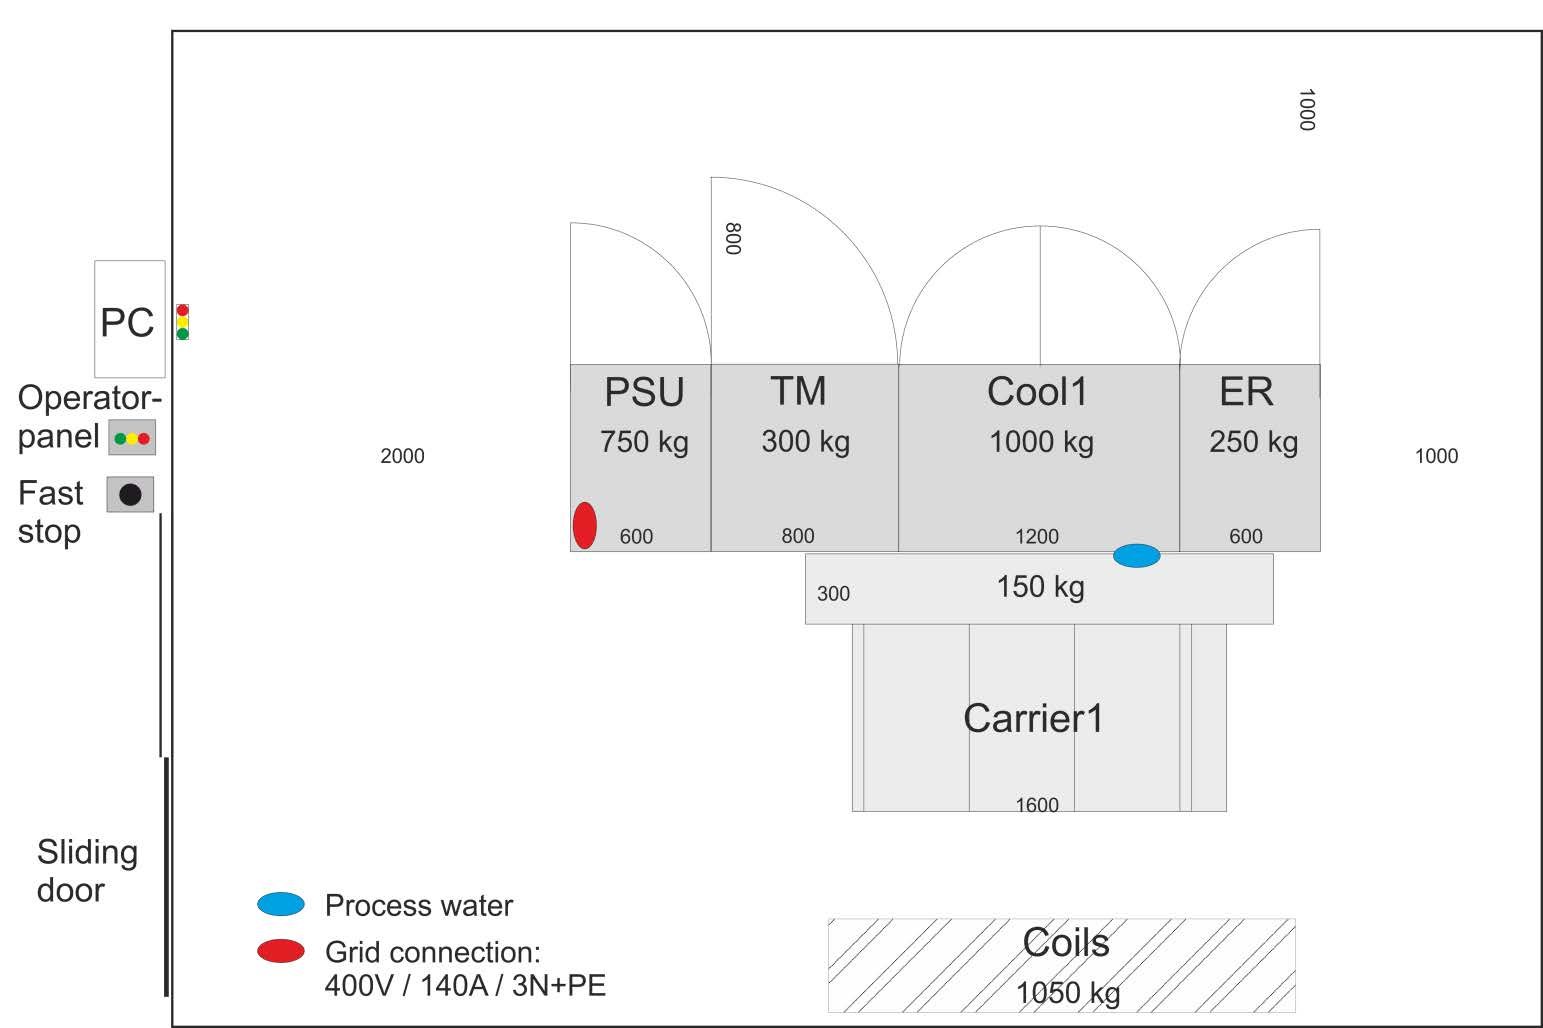
\includegraphics[width=0.8\textwidth]{Grafiken/Test Cabin}
    \caption{Aufbau des Teststandes}
    \label{fig: Aufbau des Teststandes}
    {Quelle: \cite*[7]{Main_Manuel_USTB2018}}
\end{figure}
%------------------------------------------------------------------------------------------------------
\subsubsection{Testmodule}
%------------------------------------------------------------------------------------------------------
Es gibt mehrere Testmodule, die auf dem Teststand laufen und verschiedene Funktionen der Umrichter testen.
Einige der Funktionen eines DUT können mit dem gleichen Modus eines Testmoduls überprüft werden, indem die entsprechenden Parameter ausgewählt werden.
Jeder Testablauf ist autonom und kann mehrmals ausgeführt werden, auch mit unterschiedlichen Parametern.
\\
Im Folgenden wird eine kurze Beschreibung der Funktionen der für diese Arbeit relevanten Testmodule gegeben.

Driver Consumption Test:
Der Driver Consumption Test überprüft den Stromverbrauch des Treibers im Leerlauf und während Pulssprüngen.

Pulse Test:
Der Impulstest verfügt über drei Funktionsmodi.
\begin{itemize}
    \item Im Modus \ac{FSW} kann überprüft werden, ob die Halbleiter, die sich in den \ac{DUTs} befinden, generell schalten.
    \item Im Modus \ac{OCP} kann die Überstromüberwachung weiche Kurzschlüsse überprüfen.
    Ein weicher Kurzschluss ist, wenn der Stromfluss nicht sofort und vollkommen unterbrochen wird.
    \item Im Modus \ac{DSCP} wird ein harter Kurzschluss, also ein vollständiger und sofortiger Kurzschluss, überprüft.
\end{itemize}


Power Test:
Mit diesem Test werden zwei verschiedene Funktionen getestet werden:

\begin{itemize}

    \item \ac{BIT} dient dazu, die \ac{DUTs} zyklisch zu betreiben und so reale Betriebszustände zu simulieren.
    Zudem kann mit Hilfe dieser Funktion die Kühltemperatur überprüft werden, um die korrekte Wärmeübertragung der Halbleiter sicherzustellen.
    \item Während des \ac{OTP} wird ein DUT, ähnlich wie beim \ac{BIT}, nur mit reduzierter
    Kühlung betrieben, bis die maximal zulässige Kühlkörpertemperatur erreicht ist und die Temperaturschutzschaltung auslöst.\cite*{Main_Manuel_USTB2018}

\end{itemize}

%------------------------------------------------------------------------------------------------------
\subsubsection{Testablauf}
%------------------------------------------------------------------------------------------------------
Die Schrittfolge des Testablaufes mit Montage der \ac{DUTs} ist klar festgelegt und vor jedem Durchlauf gleich.
Die Montage läuft wie folgt ab:
\begin{enumerate}

\item Die Umrichter werden auf dem Carrier befestigt. Es werden meist 3 dieser Geräte gleichzeitig getestet, Abweichungen je nach Bauform.
Die Reihenfolge der elektrischen Phasen ist bei Draufsicht des Carriers von links nach rechts U-V-W. Dies ist für das Layout des Berichtes relevant.
\item Der Kühlkreislauf wird angeschlossen, je nach Umrichtertyp Lüftungs- oder Wasserkühlung.
\item Die \ac{DUTs} werden mit den AC- und DC-Link-Kontakten verbunden, um das Gerät zu betreiben und die DC-Spannung wieder abzuleiten.
\item Das Anbringen von Signalkabeln zwischen DUT und Merkurbox. Die Merkurbox dient als Schnittstelle zwischen \ac{DUTs} und Testbench.
\item Das Montieren von VCE-Klemmen an die AC-Kontakte der \ac{DUTs}.

\end{enumerate}

Vor Beginn des Testablaufs benötigt die Test-Bench noch weitere Informationen zu den \ac{DUTs}, Testsequenzen und der Hardware-Topologie.
Diese Daten können über das Scannen von vorliegenden QR- oder Barcodes eingefügt werden.
Alternativ können diese auch über ein Eingabefenster im Teststandprogramm eingetragen werden.
Je nach Topologiekonfiguration kann auch ein zweiter Träger mit \ac{DUTs} gescannt werden,
Dies kommt bei dem Test, den das Unternehmen durchführt, nicht vor. \cite*{Main_Manuel_USTB2018}

Das eigentliche Testen mit den verschiedenen Testmodulen wird autonom durchgeführt.
Im Unternehmen läuft der Test regulär wie folgt ab:
\begin{enumerate}

\item Durchführung des Driver Consumption Testes, um die Stromversorgung der Treiberplatine auf den Umrichter zu testen.
\item Durchführung des Pulse Testes im Modus Functional-Switching, dies prüft die Umrichter.
\item Durchführung des Power Testes, in den Berichten auch XPower Test genannt.
Dieser Test simuliert die Belastung der Umrichter im Feld und überprüft,
ob sich die Werte in einem bestimmten Toleranzbereich befinden.

\end{enumerate}

Nach dem Durchlaufen eines Tests wird automatisch ein \ac{XML}-Datenfile mit den erhobenen Messdaten generiert,
die enthaltenen Messwerte und alle vorher bestimmten Einstellungen erstellt und in eine Datei eingefügt.

Bei der Demontage nach dem Testdurchlauf werden alle Schritte in umgekehrter Reihenfolge durchgeführt.
%------------------------------------------------------------------------------------------------------
\pagebreak





\subsection{Verarbeitung von XML-Daten}
\label{subsec:verarbeitung-von-xml-daten}
%------------------------------------------------------------------------------------------------------
Dieses Kapitel behandelt einige Grundlegende und für dies Arbeit relevante Aspekte von dem Dokumententype \ac{XML},
da die Messwerte bzw. die Berichte die der Testand generiert im diesem Format vorliegen.


Bei \ac{XML} handelt es sich um eine Auszeichnungssprache, also eine
formale Sprache, die verwendet werden, um die Struktur und Darstellung von Daten oder Texten zu beschreiben \cite*{Neumann2019}.
\ac{XML} wurde entwickelt, um Informationen in einem maschinenlesbaren und strukturierten Format zu speichern und zu übermitteln.
Sie wird hauptsächlich in Bereichen wie Webdiensten, Datenbanken, Konfigurationsdateien eingesetzt.
\ac{XML} ermöglicht die hierarchische Organisation von Informationen in einem strukturierten Aufbau und kann sowohl für Menschen
als auch für Maschinen interpretiert werden.\cite*{PeterBrezany2003}

Das Grundkonzept hinter \ac{XML} war, eine universelle einsetzbare und erweiterbare Sprache zu erschaffen, die von verschiedenen Systemen
unabhängig von deren grundlegenden Technologieansatz genutzt werden kann.
Hierbei ware das angestrebte Ziel Daten in einem einheitlichen Standard zwischen verschiedenen Anwendungen und Plattformen zu speichern und auszutauschen
zu kömmen.\cite*{PeterBrezany2003}
%------------------------------------------------------------------------------------------------------
\subsubsection{XML-Strukturaufbau}
%------------------------------------------------------------------------------------------------------
Eine \ac{XML}-Datei beginnt mit Prolog, der die \ac{XML}-Version und die verwendete Zeichencodierung definiert.
In Abbildung \ref{fig:XML Prolog Beispielcode} ist ein häufig genutzter Prolog dargestellt, der auch in den Teststand-Berichten genutzt wird.
Die erste Zeile des Prologs ist die sogenannte XML-Deklaration.
Die XML-Deklaration enthält häufig die Attribute sind version und encoding, jedoch nur das Attribut version ist Pflicht.
Werden auch die anderen notiert, müssen sie in der angegebenen Reihenfolge deklariert werden.
Attribut version Mit version wird die verwendete XML-Version angegeben.
Das Attribut encoding gibt die im Dokument verwendete Zeichenkodierung an, d. h. mit welcher Codierung die Datei gespeichert wird.
Fehlt die Angabe wird als Vorgabe UTF-8 (8-Bit Unicode Transformation Format) verwendet.
Neben der \ac{XML}-Deklaration können im Prolog auch noch Verarbeitungsanweisungen und Verweise auf eine \ac{DTD} deklariert werden,
dies sind jedoch optional und für diese Arbeit nicht weiter relevant.
\cite*[8,9]{Becher2022}

\begin{figure}[H]
\centering
\begin{minipage}{0.95\textwidth}
\begin{lstlisting}[language=XML]
<?xml version="1.0" encoding="UTF-8"?>
\end{lstlisting}
\end{minipage}
\caption{XML Prolog Beispielcode}
\label{fig:XML Prolog Beispielcode}
    {Quelle: eigene Darstellung}
\end{figure}


Der Hauptteil eines \ac{XML}-Dokument besteht aus einer Reihe von Elementen, die durch Tags markiert sind.
Für jedes Element gibt es ein Start- und ein EndTag, welcher das Element beginnt und beendent.
Ein Starttag kann beispeilwiese „<NamedesTags>“ so aus, dann würde der dazugehörige Endtag „</NamedesTags>“ so aussehen.
Der entscheidende Unterschied ist hierbei der Schrägstrich beim Endtag.
Der Name des Elementes wird durch den Inhalt der Keiler- und Großer-Zeichen bestimmt, bei diesem Beispiel wäre der Name „NamedesTags“.
Elemente haben einen Inhalt der aus Text, weiteren Elementen oder aus beidem bestehen kann,
wenn Elemente andere Elemente beinhalten werden Sie als Elterelemente und die enthaltenen Elemente oft Kindelemente bezeichnet.
Diese Eigenschaft der Elementente sorg dafür das XML-Datein einer hierarchischen Baumstruktur folgen.
Hierbei wird das oberste Element als Wurzelelement bezeichnet,im Englischen „root element“.\cite*[10-14]{Becher2022}


\begin{figure}[H]
\centering
\begin{minipage}{0.95\textwidth}
\begin{lstlisting}[language=XML]
<buch>
  <titel>XML-Grundlagen</titel>
  <autor>Max Mustermann</autor>
</buch>
\end{lstlisting}
\end{minipage}
\caption{XML Elemente Beispielcode}
\label{fig:XML Elemente Beispielcode}
    {Quelle: eigene Darstellung}
\end{figure}

Jedes Element kann neben Inhalt auch beliebig vielen Attributen ausgestattet sein, die zusätzliche Informationen enthalten.
Attribute werden im Start-Tag eines Elements definiert, diese bestehen immer aus eine Attributnamen und einem Wert.
Der Wert wird dabei mit Anführungszeichen deklariert, wie in Abbildung \ref{fig:XML Attribute Beispielcode} gezeigt. \cite*[10-14]{Becher2022}

\begin{figure}[H]
\centering
\begin{minipage}{0.95\textwidth}
\begin{lstlisting}[language=XML]
<buch genre="Lehrbuch">
  <titel>XML-Grundlagen</titel>
  <autor>Max Mustermann</autor>
</buch>
\end{lstlisting}
\end{minipage}
\caption{XML Attribute Beispielcode}
\label{fig:XML Attribute Beispielcode}
    {Quelle: eigene Darstellung}
\end{figure}


Kommentare werden mit den Tags „<--“ und „-->“ eingefügt und dienen der Dokumentation oder dem Hinweis auf bestimmte Teile des Codes \cite*[10-14]{Becher2022}.
Dies ist für die automatisch generierten Berichte irrelevant, jedoch für das Beschreiben der Beispiele hilfreich.
In Abbildung \ref{fig:XML Elemente Beispielcode} und Abbildung \ref{fig:XML Attribute Beispielcode} werde diese zur Beschreiben verwendet.
Kommentare werden beim Parsen des Dokuments ignoriert, parsen und Paser werden nachfolgenden Kapitel behandelt.
%------------------------------------------------------------------------------------------------------
\subsubsection{Verarbeiten von XML-Dateien}
%------------------------------------------------------------------------------------------------------
In diesem Abschnitt wird eine Zusammenfassung der grundlegenden Methoden und Techniken gegeben,
um \ac{XML}-Dateien mithilfe verschiedener Tools unabhängig von der verwendeten Programmiersprache zu verarbeiten.
Es wird beschrieben, wie man \ac{XML}-Dateien analysiert, modifiziert und überprüft, um sie für verschiedene Zwecke einsatzbereit zu machen.

Der erste Schritt beim verarbeiten einer \ac{XML}-Daten ist das Parsen.
Hierbei wird die \ac{XML}-Datei in ein Programm geladen und in ein Format umgewandelt, das das Programm interpretieren kann.
XML-Paser prüfen hierbei auch die \ac{XML}-Daten auf Korrektheit, also ob die Voralien eingehalten werden und das Dokument vollständig ist.
Dabei wird in nicht-validierte Parser und validierende Paser differenziert.
Der Unterschied besteht dadrin, dass validierte Paser neben der  korrekte Schachtelung und Bezeichnung der Strukturelemente
wie die nicht-validierten Paser auch noch auf eine Vorgabe einer Dokumenttypdefinition oder eines Schemas prüfen.\cite*[10]{Becher2022}

Paser werden verwendet um eine Applikation über eine \ac{API} eine Schnittstelle auf ein \ac{XML}-Dokument zu geben.
Bei \ac{API}s wird in diesem Bereich zwischen zwei Grundtypen unterschieden:\cite*[405]{Becher2022}

Die baumbasierten \ac{API}s lesen über den XML-Parser das XML-Dokument ein,
parst es und erzeugt ein Modell als Baum von Knoten im Arbeitsspeicher.
Auf Grunde der im XML-Dokument vorkommenden Informationseinheiten wird in verschiedene Knotentypen unterschieden.
Das generierte Modell dient der Applikation für die weitere anwendungsspezifische Verarbeitung.
Ein Beispiel für eine baumbasierte \ac{API}s ist \ac{DOM}.

\ac{DOM}ist Ein objektorientiertes Modell, das die Struktur eines XML-Dokuments abbildet.
In der Baumstruktur wird das gesamte Dokument abgebildet, indem jedes Element, Attribut und jeder Text bzw. Inhalt als Knoten gilt.
Das DOM hat den Vorteil, dass es das \ac{XML}-Dokument vollständig im Arbeitsspeicher darstellt, was das Durchsuchen und Bearbeiten des Dokuments erleichtert.
Zudem bittet es eine einfache Schnittstelle bereitstellt, um XML-Daten zu erreichen und zu verändern.
Allerdings benötigt diese Herangehensweise viel Speicherplatz,
da es das gesamte Dokument im Arbeitsspeicher ablegt, was bei großen \ac{XML}-Dokumenten ein Problem darstellen kann.\cite*[413,414]{Becher2022}


Die ereignisbasierten \ac{API}s lesen \ac{XML}-Dokument sequenziell von begin durch
ein und meldet während des Lesens jedes Ereignis durch sogenannte Callbacks an die aufrufende Applikation zurück.
Ein Ereignis ist ein Signal, das Änderungen in dem Markup-Status anzeigt.
Das Bedeutet Ereignise tritten bei Element-Tags, Zeichendaten, Kommentaren, Verarbeitungsanweisungen, sowie bei den Grenzen des Dokumentes auf.
Der Parser sendet hierbei durch die Callbacks eine Mitteilung an die aufrufende Applikation, welche Ereignisse eingetreten sind.
Das Programm, das den Parser aufgerufen hat, muss nun das Ereignis interpretieren und entsprechend reagieren.
Das \ac{XML}-Dokument wird hierbei nicht vollständig im Arbeitsspeicher gespeichert, sondern in Teilen gelesen und bearbeitet.
Deshalb eignen sich ereignisbasierte \ac{API}s besonders gut für die Verarbeitung großer \ac{XML}-Dateien, da dies für eine geringe Arbeitsspeicherbelastung sorgt.
Trotz der Effizienz hinsichtlich des Speicherverbrauchs sind ereignisbasierte \ac{API}s für die Datenmanipulation nicht sonderlich gut geeignet.
Es wird nämlich durch das Teileweise einlesen keine umfassende Dokumentstruktur wie beim aufgebaut Die baumbasierten \ac{API}s,
welches die Manipulation bzw. bearbeitung erschwert.
Ein Beispiel für eine große ereignisbasierte \ac{API} ist \ac{SAX}.
Diese \ac{API} abreitet nach dem oben beschriebenen Prinzip und wurde ursprünglich als Java-\ac{API} entwickelt, inzwischen gibt es \ac{SAX} auch für weiter Sprachen wie
z. B. C++, Perl und Python.\cite*[405]{Becher2022}

Neben diesen beide großen Beispielen gibt es auch einige kleiner Anbieter mit abgewandelten Methoden,
die jedoch in dem Umfang deutlich kleiner gehalten sind und weniger Funktionen bitten.
Ein Beispiel dafür wäre ElementTree.
ElementTree ist eine unkomplizierte und minimalistische Python-Bibliothek, die für die Bearbeitung von \ac{XML} genutzt wird.
Sie präsentiert eine Baumstruktur, die das \ac{XML}-Dokument effektiv darstellt und einfache Techniken zum Durchsuchen,
Modifizieren und Erstellen von \ac{XML}-Dokumenten bietet.\cite*{ElementTree2025}

lxml
\pagebreak

\subsection{Flask-Grundlagen und Funktionsweise}\label{subsec:flask-grundlagen-und-funktionsweise}

In diesem Unterkapitel wird das Webframework Flask, das in der Web-Applikation genutzt wird, behandelt.
Ein grundlegender Überblick wird gegeben und sein wichtiger Funktionsablauf wird erläutert.

\subsubsection{Überblick}

Flask ist ein schlankes Webframework für Python, das auf WSGI (Web Server Gateway Interface) basiert.
Das Web Server Gateway Interface (WSGI) ist eine Schnittstelle, die es Webservern ermöglicht, mit Python-Webanwendungen oder -Frameworks zu kommunizieren.  Der Begriff „leichtgewichtiges“ bedeutet in diesem Zusammenhang, dass der Framework-Kern mit Bedacht minimalistisch entworfen wurde und viele Funktionen nur durch Erweiterungen hinzugefügt werden können.
In der Standardkonfiguration setzt sich Flask aus zwei zentralen Komponenten zusammen: \cite{FlaskDocumentation}
\begin{itemize}

    \item Werkzeug: Ist eine Sammlung von Funktionen zum Erstellen von WSGI-Anwendungen, die HTTP-Requests und -Responses abstrahiert und die Schnittstelle zwischen dem Webserver und der Python-Anwendung ermöglicht.  Außerdem umfasst sie Funktionen zum Aufspüren und Beheben von Fehlern (Debugging), zum Zuordnen von URLs zu Funktionen oder Aktionen in einer Webanwendung (URL-Routing) sowie Hilfsfunktionen für die Arbeit mit HTTP (HTTP-Utilities).

    \item Jinja2: eine Template-Engine, die es ermöglicht, HTML-Dateien mit Platzhaltern, Schleifen, Bedingungen und weiteren Syntaxelementen zu erstellen, um sie dynamisch in der Anwendung zu rendern. Sie erlaubt so die dynamische Erstellung von HTML-Seiten (oder anderen Textdateien), indem Python-Daten in Platzhalter innerhalb einer Vorlage (Template) eingefügt werden.

\end{itemize}


\subsubsection{Grundprinzip der Funktionsweise}

Die beiden obengenannten zentralen Komponenten bilden die Grundlagen für die Funktionsweise von Flask.

Für die Darstellung im Browser werden die Seiten der Applikation serverseitig dynamisch erstellt und an den Client gesendet, indem diese Template-Vorlagen genutzt werden.
Die HTTP-Anfragen (Requests) des Clients werden über die WSGI-Schnittstelle, die Werkzeug bereitstellt, entgegengenommen, von der Anwendung verarbeitet und als HTTP-Antworten (Responses) an den Webserver zurückgeschickt. Hierbei kümmert sich Jinja2 um die dynamische Erstellung der HTML-Seiten, während Werkzeug die Kommunikation zwischen Webserver und Anwendung regelt. Die Auslieferung von dynamisch generierten Webseiten wird durch das Zusammenwirken dieser beiden Komponenten ermöglicht.

Um die Funktionsweise von Flask zu veranschaulichen, wird im Folgenden ein typischer Ablauf einer Webanfrage kurz beschrieben: \cite{FlaskLifecycle,Kennedy2024_FlaskRequests}
\begin{enumerate}

    \item \textbf{Erhalt einer HTTP-Anfrage}\\
Ein Webclient (wie ein Browser) schickt eine Anfrage an den Webserver, der sie über die WSGI-Schnittstelle an die Flask-Anwendung weiterleitet.

    \item \textbf{Routing}\\
Flask untersucht die URL und weist sie einer passenden View-Funktion zu.  Dies erfolgt über sogenannte Routen, die mit dem Dekorator @app.route() festgelegt werden.

    \item \textbf{Bearbeitung der Anfrage}\\
Die Geschäftslogik wird in der zugeordneten Funktion ausgeführt; dazu gehört unter anderem das Auslesen von Parametern, der Zugriff auf eine Datenbank oder die Aufbereitung von Daten.

    \item \textbf{Template Rendering (optional)}\\
Falls die Antwort HTML-basiert ist, wird ein Jinja2-Template mit dynamischen Daten gefüllt und gerendert.

    \item \textbf{Erzeugung der HTTP-Antwort}\\
Flask gibt die fertige Antwort (z. B. HTML, JSON oder Redirect) an den Client zurück.

\end{enumerate}


\subsubsection{Blueprints in Flask}

Flask ermöglicht es, über interne Funktionen und Klassen sogenannte Blueprints zu erstellen und zu nutzen.
Blueprints sind eine strukturierte Möglichkeit, Webanwendungen modular aufzubauen.
Ein Blueprint stellt ein logisches Teilmodul der Anwendung dar und kann eigene Routen, Templates, statische Dateien und Logik enthalten.
Dadurch lassen sich umfangreiche Projekte in klar abgegrenzte Funktionsbereiche unterteilen, was die Übersichtlichkeit und Wartbarkeit der Anwendung erhöht.
Jeder Blueprint wird in einer separaten Datei definiert und anschließend in der Hauptapplikation registriert.
Dieses Vorgehen ermöglicht es, neue Funktionsmodule ohne Eingriff in bestehende Komponenten zu ergänzen.
Somit befördert Blueprint das Unterteilen in modulare Softwarearchitektur, insbesondere die geringe Kopplung und hohe Kohäsion zwischen den Modulen.\cite{FlaskBlueprints}







\subsection{Datenbankentwurf und Normalisierung}
\label{subsec:datenbankentwurf-und-normalisierung}
%------------------------------------------------------------------------------------------------------
Datenbanken sind strukturierte Zusammenstellungen von Daten, die elektronisch gespeichert und verwaltet werden.
Ihr Hauptziel ist es, große Datenmengen strukturiert zu speichern, den Zugriff zu optimieren und die Integrität der Daten zu gewährleisten.
Datenbanken haben im Vergleich zu anderen Dateisystemen Mechanismen, die mehreren Benutzern die parallele Nutzung ermöglichten,
sowie redundante Datenhaltung vermeiden und die effiziente Abfragen über spezielle Sprachen wie die \ac{SQL} ermöglichen.

Um den unterschiedlichen Anforderungen an Konsistenz, Flexibilität und Skalierbarkeit gerecht zu werden, ist es unerlässlich
, bei der Entwicklung moderner Informationssysteme relationale Datenbanken, dokumentenbasierte Systeme oder hybride Modelle zu verwenden.


%------------------------------------------------------------------------------------------------------
\subsubsection{Datenbankstruktur}
%------------------------------------------------------------------------------------------------------
Die Struktur der Datenbank legt fest, wie das Datenbanksystem organisiert ist und wie die Datenelemente angeordnet sind.
Das Grundprinzip relationaler Datenbanken sind im Grunde Tabellen und die Beziehungen zwischen diesen.
Die Hauptbestandteile sind:

\begin{itemize}
\item Tabellen – das grundlegende Element, welches Daten in Zeilen (Tupeln) und Spalten (Attributen) strukturiert.
\item Ein Datensatz in einer Tabelle wird durch Primärschlüssel (Primary Keys) eindeutig identifiziert.
\item Schlüssel aus anderen Tabellen (Foreign Keys)  Tabellenverknüpfung, um die referenzielle Integrität zu gewährleisten.
\item Indizes: Datenstrukturen, die das Beschleunigen von Abfragen ermöglichen.
\item Views: sie sind virtuelle Tabellen und beruhen auf den Ergebnissen von Abfragen.
\item Constraints: Vorgaben zur Gewährleistung der Datenintegrität (z.B. Wertebereiche, Pflichtfelder oder Dopplungen).
\end{itemize}
%------------------------------------------------------------------------------------------------------
\subsubsection{Datenintegrität und Normalisierung}
%------------------------------------------------------------------------------------------------------
Ein methodischer Ansatz zur Reduzierung von Redundanzen und Anomalien ist die Normalisierung.
Der Prozess erfolgt schrittweise durch die Normalformen, die durch Indizes  (1NF, 2NF, 3NF, BCNF) definiert sind.
Alle Normalformen haben spezifische Arten von Datenanomalien zum Ziel:

\begin{itemize}

\item 1. Normalform (1NF): Beseitigung mehrfacher Werte innerhalb einer Zelle;  atomare Attribute.
\item 2. Normalform (2NF): Beseitigung partieller Abhängigkeiten.
\item 3. Normalform (3NF): Beseitigung transitiver Abhängigkeiten.

\end{itemize}

Die Gewährleistung, dass Daten korrekt, konsistent und vollständig sind,
fällt unter das Konzept der Datenintegrität.
Sie wird erzielt durch:

\begin{itemize}
\item
Entity-Integrität (eindeutige Primärschlüssel).
\item
Referentielle Integrität (gültige Fremdschlüsselverweise).

\item Domänenintegrität (gültige Wertebereiche und Datentypen).
\item Entity-Integrität (eindeutige Primärschlüssel).
\item Referentielle Integrität (gültige Fremdschlüsselverweise).
\item Integrität der Domäne (gültige Wertebereiche und Datentypen).

\end{itemize}

%------------------------------------------------------------------------------------------------------
\subsubsection{Vorgehen zur Erstellung der Datenbank}
%------------------------------------------------------------------------------------------------------
Bei der Erstellung einer Datenbank sollte nach folgendem Schema vorgegangen werden.
Bei diesem Schema gilt es, sowohl technische als auch konzeptionelle Aspekte zu berücksichtigen:

\begin{enumerate}

\item
Anforderungsanalyse

Zuerst wird im Hinblick auf das Geschäftsumfeld bestimmt, welchen konkreten Zweck die Datenbank erfüllen soll.
Hierbei ist die Zweckbestimmung  entscheidend, da sie festlegt, welche Daten als relevant gelten.
Der Konzeptvorschlag, der das Projektziel definiert und die Vorgehensweise umreißt, ist das Ergebnis.
\begin{itemize}

\item
Festlegung der fachlichen und technischen Voraussetzungen.
\item
Bestimmung der relevanten Datenquellen und -formate.
\item
Definition von Integritäts- und Sicherheitsanforderungen.

\end{itemize}

\item
Konzeptionelles Datenmodell

Es soll das geschäftliche Umfeld betrachtet werden.
Die bestehende Objekte (z.B. Reports mit Materialnummer, Datum, Version), deren Attribute sowie die Beziehungen und Einschränkungen zwischen diesen Objekten.
Das Entity-Relationship-Modell (ERM) nach Chen oder das PrecisedERM (PERM) werden häufig zur Modellierung verwendet.
Der konzeptionelle Entwurf ist die Grundlage für die nächste Phase und dient als Diskussionsgrundlage.
\begin{itemize}

\item Die Entwicklung eines Entity-Relationship-Modells (ERM), das die reale Welt in Entitäten, Attribute und Beziehungen abbildet.
\item Die Einbeziehung von Kardinalitäten (1:1, 1:n, n:m).

\end{itemize}

\item
Logisches Datenmodell

Der konzeptionelle Entwurf wird in einen logischen Entwurf umgewandelt, der die fachlichen Konzepte in ein datenbanktechnisches Format überführt.
In der Regel kommt das Relationenmodell zum Einsatz, welches die Daten in Form von Tabellen organisiert.
Transformationsregeln garantieren, dass Beziehungen und Integritätsbedingungen richtig umgesetzt werden.
\begin{itemize}

\item Transformation des konzeptionellen Modells in ein relationales Schema.
\item Festlegung von Tabellen, Spalten (Attribute), Primärschlüsseln und Fremdschlüsseln.
\item Definition von Datentypen und Zellenkofigurationen (z.B. NOT NULL, UNIQUE, CHECK).
\end{itemize}

\item
Physisches Datenmodell

Eine physische Datenbankstruktur wird durch \as{SQL} erstellt, basierend auf dem logischen Entwurf.
Die konkrete Festlegung von Tabellen, Indizes, Constraints usw. erfolgt dabei durch  Das System,
das wir implementiert haben, wird immer wieder getestet und zusammen mit den Nutzerinnen auf fachliche Richtigkeit überprüft.
\begin{itemize}

\item Realisierung des logischen Modells in einer spezifischen Datenbankmanagementsoftware (z.B. MySQL, Mariadb oder Microsoft SQL Server).er).
\item Die Verbesserung der Speicherstrukturen, der Indexierung und der Partitionierung.

\end{itemize}

\item
Implementierung und Prüfung

Nach der erfolgreichen Umsetzung wird das System vom Kunden gemäß einem vorher festgelegten Abnahmeplan freigegeben.
Ein Wartungsplan kümmert sich anschließend um die Betreuung, schult die Endbenutzer und überwacht die IT-Umgebung kontinuierlich.
\begin{itemize}

\item Den Aufbau der Tabellen und Relationen entsprechend dem Datenbankschema.

\item Die Testdaten implementieren.

\item Die Kontrolle der Funktionalität und Leistung.

\end{itemize}

\end{enumerate}

\pagebreak


\subsection{Grundlagen der Datenvisualisierung}
\label{subsec:grundlagen-der-datenvisualisierung}

\subsubsection{Begriff und Zielsetzung}

Unter Datenvisualisierung wird die visuelle Aufbereitung von Daten verstanden, um Muster, Trends, Zusammenhänge
oder Anomalien erkennbar zu machen.
Sie stellt ein zentrales Hilfsmittel dar, um komplexe Informationen effizient zu kommunizieren und kognitive
Verarbeitungsprozesse zu unterstützen[Shneiderman, 1996].
Durch die grafische Darstellung wird es dem Betrachter ermöglicht, große Datenmengen intuitiv zu erfassen,
ohne ausschließlich auf numerische oder textuelle Formen angewiesen zu sein.
Die Zielsetzung der Datenvisualisierung umfasst in der Regel drei Kernaspekte[Ware, 2021]:

\begin{enumerate}

\item
Exploration: Unterstützung bei der Entdeckung neuer Zusammenhänge und Hypothesen.
\item
Analyse: Erleichterung der detaillierten Untersuchung von Strukturen und Abhängigkeiten.
\item
Kommunikation: Vermittlung von Ergebnissen an unterschiedliche Zielgruppen.

\end{enumerate}

\subsubsection{Theoretische Grundlagen}

Die Grundlage wirksamer Datenvisualisierung liegt in der menschlichen Wahrnehmungspsychologie.
Insbesondere die Gestaltungsgesetze (z.B. Gesetz der Nähe, Ähnlichkeit und Kontinuität) spielen eine zentrale Rolle,
da sie bestimmen, wie Informationen visuell gruppiert und interpretiert werden[Wertheimer, 1923].

Zusätzlich beschreibt die Theorie der \textit{kognitiven Belastung} (Cognitive Load Theory),
dass Darstellungen so gestaltet werden sollten, dass sie die Arbeitsgedächtniskapazität nicht überlasten[Sweller, 1988].


Ein weiterer theoretischer Rahmen ist Shneidermans Visual Information-Seeking Mantra:



„Overview first, zoom and filter, then details-on-demand.“

Dieses Prinzip betont die Notwendigkeit einer schrittweisen Annäherung an Daten, um vom Gesamtüberblick bis hin zu
spezifischen Details zu gelangen.


\subsubsection{Formen der Datenvisualisierung}

Datenvisualisierungen lassen sich in verschiedene Kategorien einteilen[Few, 2012]:

\begin{itemize}

\item
Explorative Visualisierung: Interaktive Darstellungen, die zur Untersuchung und Hypothesengenerierung dienen.
\item
Explikative Visualisierung: Fokussierte, oft statische Darstellungen, die Ergebnisse gezielt kommunizieren.
\item
Interaktive Dashboards: Kombination mehrerer Visualisierungstypen, häufig für Monitoring und Entscheidungsunterstützung.

\end{itemize}

Je nach Datentyp und Analyseziel kommen unterschiedliche Diagrammformen und Techniken zum Einsatz:

\begin{itemize}

\item
Zeitreihen: Liniendiagramme, Flächendiagramme
\item
Kategorische Daten: Balken- und Säulendiagramme
\item
Zusammenhänge: Streudiagramme, Blasendiagramme
\item
Verteilungen: Histogramme, Boxplots
\item
Hierarchien und Netzwerke: Baumdiagramme, Graphvisualisierungen

\end{itemize}

\subsubsection{Qualitätskriterien}

Eine gute Datenvisualisierung erfüllt folgende Kriterien[Tufte, 2001]:


\begin{itemize}

\item
Klarheit: Vermeidung unnötiger grafischer Elemente („Chartjunk“)
\item
Genauigkeit: Wahrheitsgetreue Darstellung ohne Verzerrung von Skalen oder Proportionen
\item
Effizienz: Schnelle Erfassbarkeit der relevanten Information
\item
Ästhetik: Ansprechende Gestaltung zur Förderung der Akzeptanz
\item
Barrierefreiheit: Berücksichtigung farbsehschwacher Nutzer durch geeignete Farbpaletten

\end{itemize}

\subsubsection{Technologische Aspekte}

Mit dem Fortschritt moderner IT-Systeme haben sich leistungsfähige Werkzeuge und Bibliotheken für die
Datenvisualisierung etabliert.
Beispiele sind Matplotlib und Plotly im Python-Umfeld, D3.js im Webbereich.

In Webapplikationen ermöglichen interaktive Bibliotheken eine nahtlose Einbettung in Benutzeroberflächen,
wodurch sowohl explorative als auch explikative Ziele unterstützt werden.

\subsubsection{Graphen erstellung mit JS}


\subsection*{Chart.js}

Eine einfache und beliebte Bibliothek für Standarddiagramme wie Balken, Linien oder Kreisdiagramme. Schnell eingebunden, gute Standardoptik, ideal für kleinere Projekte oder schnelle Visualisierungen.



\subsection*{D3.js}

Eine sehr mächtige Low-Level-Bibliothek, die mit SVG, Canvas und HTML arbeitet. Extrem flexibel für individuelle und interaktive Visualisierungen, aber mit einer steilen Lernkurve.



\subsection*{Plotly.js}

Bietet viele interaktive Diagramme (Zoom, Hover, Export als PNG). Unterstützt auch 3D- und wissenschaftliche Charts. Gut geeignet für Dashboards und Datenanalyse.



\subsection*{ECharts (Apache ECharts)}

Eine leistungsstarke Open-Source-Bibliothek von Apache. Unterstützt viele Diagrammtypen (inkl. Heatmaps, Maps, Candlesticks) mit Animationen und Interaktivität. Besonders beliebt für komplexe Enterprise-Web-Apps.



\subsection*{Highcharts}

Eine professionelle, kommerzielle Lösung (kostenlos für private Nutzung). Sehr einfach konfigurierbar, liefert Business-taugliche Diagramme mit vielen Optionen. Oft in Unternehmen eingesetzt.



\subsection*{vis.js}

Spezialisiert auf Netzwerk- und Zeitachsenvisualisierungen. Eignet sich besonders für Knoten-Graphen, Beziehungen oder Prozessdiagramme mit Interaktivität.



\subsection*{Recharts}

Eine React-spezifische Bibliothek, die auf D3.js basiert. Bietet eine einfache Komponenten-API für gängige Diagramme. Ideal, wenn deine Web-App mit React entwickelt ist.



\pagebreak



\section{Anforderungen an modulare Softwareentwicklung (nach ISO/IEC 9126)}
\label{sec:anforderungen-an-modulare-softwareentwicklung-(nach-iso/iec-9126)}

Die Norm \textbf{ISO/IEC 9126} beschreibt ein Qualitätsmodell für Softwareprodukte, das mehrere Haupt- und Untermerkmale definiert.
Diese Merkmale lassen sich auf die modulare Softwareentwicklung übertragen, da sie zentrale Eigenschaften wie Wartbarkeit, Erweiterbarkeit und Austauschbarkeit quantifizierbar machen.
Eine modulare Architektur erfüllt diese Qualitätsziele durch klar definierte Schnittstellen, lose Kopplung und eine hohe Kohäsion der Module.\cite{ISOIEC9126-1991}

\begin{itemize}
    \item \textbf{Funktionalität:}
    Jedes Modul soll die vorgesehenen Aufgaben korrekt und zweckmäßig ausführen.
    Eine hohe Funktionalität setzt voraus, dass Module die geforderten Spezifikationen erfüllen, interoperabel mit anderen Komponenten sind und relevante Standards einhalten.
    \emph{Untermerkmale: Eignung, Korrektheit, Interoperabilität, Konformität, Sicherheit.}

    \item \textbf{Zuverlässigkeit:}
    Module sollen auch unter unerwarteten Bedingungen stabil arbeiten und definierte Wiederherstellungsmechanismen besitzen.
    Eine hohe Zuverlässigkeit gewährleistet, dass Fehlfunktionen lokal begrenzt bleiben und das Gesamtsystem funktionsfähig bleibt.
    \emph{Untermerkmale: Reife, Fehlertoleranz, Wiederherstellbarkeit.}

    \item \textbf{Benutzbarkeit:}
    Module und Schnittstellen sollen verständlich, erlernbar und bedienbar sein.
    Diese Anforderung gilt sowohl für Benutzerschnittstellen als auch für APIs, um eine konsistente Integration und Nutzung zu ermöglichen.
    \emph{Untermerkmale: Verständlichkeit, Erlernbarkeit, Bedienbarkeit.}

    \item \textbf{Effizienz:}
    Module sollen vorhandene Ressourcen optimal nutzen und geforderte Leistungswerte einhalten.
    Eine effiziente Implementierung trägt zu einem stabilen Laufzeitverhalten und einer guten Skalierbarkeit des Gesamtsystems bei.
    \emph{Untermerkmale: Zeitverhalten, Ressourcenverhalten.}

    \item \textbf{Wartbarkeit:}
    Module sollen leicht analysierbar, anpassbar und testbar sein.
    Änderungen müssen möglichst lokal vorgenommen werden können, ohne unbeabsichtigte Auswirkungen auf andere Systemkomponenten zu verursachen.
    \emph{Untermerkmale: Analysierbarkeit, Änderbarkeit, Stabilität, Testbarkeit.}

    \item \textbf{Portabilität:}
    Module sollen an unterschiedliche Zielumgebungen anpassbar und bei gleichbleibender Schnittstelle austauschbar sein.
    Dadurch wird die Wiederverwendung und langfristige Nutzbarkeit der Software verbessert.
    \emph{Untermerkmale: Anpassbarkeit, Installierbarkeit, Konformität, Austauschbarkeit.}
\end{itemize}

Die Berücksichtigung dieser Qualitätsmerkmale bei der Entwicklung modularer Systeme stellt sicher, dass Software langfristig wartbar, erweiterbar und zuverlässig bleibt.
Das Qualitätsmodell der ISO/IEC 9126 bietet damit eine strukturierte Grundlage zur Bewertung und Verbesserung der architektonischen Qualität modularer Anwendungen. \cite{ISOIEC9126-1991}


\pagebreak

%! Author = jbf
%! Date = 31.07.25
\newpage
\section{Analyse und Konzeption}
\label{sec:analyse-und-konzeption}


In diesem Kapitel werden die grundlegenden Anforderungen und konzeptionellen
Überlegungen für die Entwicklung der Webapplikation beschrieben.
Ziel ist es, eine fundierte Basis für die spätere Implementierung zu schaffen, indem sowohl die
funktionalen als auch die nicht-funktionalen Anforderungen analysiert und geeignete technische Konzepte erarbeitet werden.
Dazu werden zunächst die Ausgangssituation und die zu verarbeitenden Datenquellen untersucht.
Die erarbeiteten Konzepte bilden die Grundlage für das Design und die Realisierung der Software im weiteren Verlauf der Arbeit.


\subsection{Definition der Anforderungen}
\label{sec:definition-der-anforderungen-und-ihre-interpretation}

In diesem Abschnitt werden die funktionalen und nicht-funktionalen Anforderungen der zu entwickelnden Web-Applikation beschrieben.
Sie wurden in Abstimmung mit den späteren Nutzerinnen und Nutzern sowie den betreuenden Personen im Unternehmen festgelegt.
Die Anforderungen bilden die Grundlage für den Entwurf und die Umsetzung der Software und dienen dazu, deren Zielsetzung, Funktionsumfang und technische Rahmenbedingungen klar zu definieren.


\subsubsection{Funktionale Anforderungen}\label{subsec:funktionale-anforderungen}

Die funktionalen Anforderungen beschreiben die vorgesehenen Funktionen und Abläufe der Applikation.
Sie definieren, was die Anwendung leisten soll und wie die Nutzerinnen und Nutzer mit ihr interagieren können.

\begin{enumerate}
  \item Navigation und Benutzerführung \\
  Die Applikation soll eine einfache und übersichtliche Navigation ermöglichen.
  Der Wechsel zwischen den Hauptfunktionen erfolgt über eine feststehende Menüleiste im oberen Bereich der Benutzeroberfläche.
  Dadurch können die Bereiche Upload, Berichte und Analyse direkt aufgerufen werden.

  \item Einlesen von XML-Dateien \\
  Das Einlesen der automatisch generierten XML-Berichte erfolgt über eine Upload-Seite.
  Die Anwendung soll sowohl ältere als auch neuere XML-Strukturen verarbeiten können, da der Teststand unterschiedliche Versionen erzeugt.

  \item Datenverarbeitung und Speicherung \\
  Nach dem Upload sollen die XML-Dateien automatisch geparst, validiert und in die Datenbank überführt werden.
  Doppelte Einträge sollen erkannt und vermieden werden.

  \item Anzeige der Berichte \\
  Die gespeicherten Berichte sollen tabellarisch dargestellt werden.
  Jede Zeile repräsentiert einen Testbericht und zeigt die wichtigsten Informationen wie Datum, Seriennummer, Materialnummer und Testergebnis an.

  \item Filter- und Suchfunktionen \\
  Die Berichtstabelle soll über Filteroptionen verfügen, um gezielt nach bestimmten Kriterien
  (z.\,B. Datum, Seriennummer, Testmodul oder Ergebnisstatus) zu suchen.

  \item Grafische Darstellung der Testdaten \\
  Die Anwendung soll die Messergebnisse der einzelnen Module grafisch darstellen.
  Die Diagramme sind nach Modulen sortiert und enthalten eine klare Achsenbeschriftung sowie Legenden.
  Das Layout der Diagramme soll sich an den Graphen des Teststandprogramms orientiert, um den Nutzerinnen und Nutzern die Interpretation zu erleichtern.

  \item Systemmeldungen und Fehlermanagement \\
  Nach erfolgreichen oder fehlerhaften Aktionen (z.\,B. Upload, Datenbankeintrag, Filterabfrage) sollen entsprechende Systemmeldungen angezeigt werden, um den Benutzerstatus transparent zu machen.

  \item Exportfunktionen \\
  Die Anwendung soll die Möglichkeit bieten, ausgewählte Graphen in ein externes Format zu exportieren.
  Dadurch können die Graphen auch außerhalb der Anwendung weiterverarbeitet werden.
\end{enumerate}

\subsubsection{Nicht-funktionale Anforderungen}
\label{subsec:nicht-funktionale-anforderungen}

Die nicht-funktionalen Anforderungen beschreiben die Qualitätsmerkmale der Software.
Sie legen fest, unter welchen Bedingungen die Applikation betrieben werden soll und welche Eigenschaften sie erfüllen muss.

\begin{enumerate}
  \item Plattform und Laufzeitumgebung \\
  Die Web-Applikation wird auf einem unternehmenseigenen Apache2-Server betrieben.
  Sie basiert auf Python und dem Webframework Flask.

  \item Performance \\
  Das System muss auch bei größeren XML-Dateien zuverlässig arbeiten.
  Hierbei wird von XML-Daten mit einer Vielzahl von Testmodulen ausgegangen.
  Eine aktive Laufzeitoptimierung ist nicht erforderlich, solange der Arbeitsfluss nicht beeinträchtigt wird.

  \item Usability \\
  Die Benutzeroberfläche soll intuitiv bedienbar sein und eine klare Struktur aufweisen.
  Eingabefehler sollen vermieden und, wenn möglich, automatisch erkannt werden.

  \item Modularität und Wartbarkeit \\
  Die Applikation ist modular aufgebaut, um eine einfache Pflege und spätere Erweiterung zu ermöglichen.
  Änderungen an einzelnen Komponenten sollen keine Anpassungen an anderen Modulen erfordern.

  \item Sicherheit und Datenintegrität \\
  XML-Dateien müssen vor dem Einlesen auf korrekte Struktur und mögliche Sicherheitsrisiken geprüft werden
  (z.\,B. Schutz vor fehlerhaften oder manipulierten Dateien).

  \item Fehler- und Ausnahmebehandlung \\
  Unerwartete Systemfehler sollen abgefangen und im Log gespeichert werden.
  Für Benutzerinnen und Benutzer werden stattdessen verständliche Fehlermeldungen ausgegeben.

  \item Skalierbarkeit \\
  Das System soll bei Bedarf mit minimalem Aufwand um zusätzliche Funktionen, Testmodule oder Datenquellen erweitert werden können.

  \item Kompatibilität \\
  Die Applikation soll auf allen gängigen Browsern lauffähig sein (z.\,B. Chrome, Edge, Firefox).

  \item Dokumentation und Nachvollziehbarkeit \\
  Der Code soll übersichtlich dokumentiert werden.
  Wichtige Abläufe (Upload, Datenverarbeitung, Visualisierung) werden nachvollziehbar beschrieben.
\end{enumerate}

\subsubsection{Anforderungen an die Datenbank}
\label{subsec:anforderungen-an-die-datenbank}

Die Datenbank ist ein zentraler Bestandteil der Anwendung.
Sie speichert alle relevanten Testdaten, Parameter und Informationen aus den XML-Berichten.

\begin{enumerate}

  \item Datenbanksystem \\
  Die Datenbank basiert auf dem relationalen Datenbanksystem MariaDB.

  \item Vollständige Abbildung der XML-Daten \\
  Sie muss in der Lage sein, sämtliche in den XML-Berichten enthaltenen Daten vollständig abzubilden,
  um die Wiederherstellung eines gesamten Testberichts theoretisch zu ermöglichen.

  \item Vermeidung von Datendopplungen \\
  Datendopplungen sollen vermieden werden.
  Häufig vorkommende Informationen (z.\,B. Teststandname, Versionsnummern, DUT-Typen) werden ausgelagert und über Fremdschlüssel referenziert.

  \item Strukturierung von Gerätedaten \\
  Für DUT-Typen und Seriennummern werden separate Informationstabellen angelegt,
  um Redundanzen zu vermeiden und die Datenstruktur klar zu halten.

  \item Erweiterbarkeit der Datenbankstruktur \\
  Die Datenbankstruktur soll so gestaltet sein, dass zukünftige Teststände oder zusätzliche Testmodule problemlos integriert werden können.

  \item Versionierung und Migration \\
  Änderungen an der Datenbankstruktur werden verwaltet,
  um eine konsistente Weiterentwicklung der Datenbank sicherzustellen.

  \item Datenvalidierung und Konsistenzprüfung \\
  Beim Einfügen neuer Datensätze sollen Validierungen sicherstellen,
  dass die Werte logisch und formal korrekt sind (z.\,B. keine Nullwerte bei Pflichtfeldern, korrekte Datentypen).
\end{enumerate}

Die beschriebenen Anforderungen bilden den Rahmen für die Entwicklung der Web-Applikation.
Während die funktionalen Anforderungen die konkreten Aufgaben und Abläufe definieren,
legen die nicht-funktionalen Anforderungen fest, wie die Anwendung qualitativ umgesetzt werden soll.
Zusammen mit den Datenbankanforderungen bilden sie die Grundlage für den folgenden Entwurf der Systemarchitektur und die spätere Implementierung.

\subsection{Grundlegender Ablauf des Programmes}
\label{subsec:grundlegender-ablauf-des-programmes}

\begin{figure}[H]
    \centering
    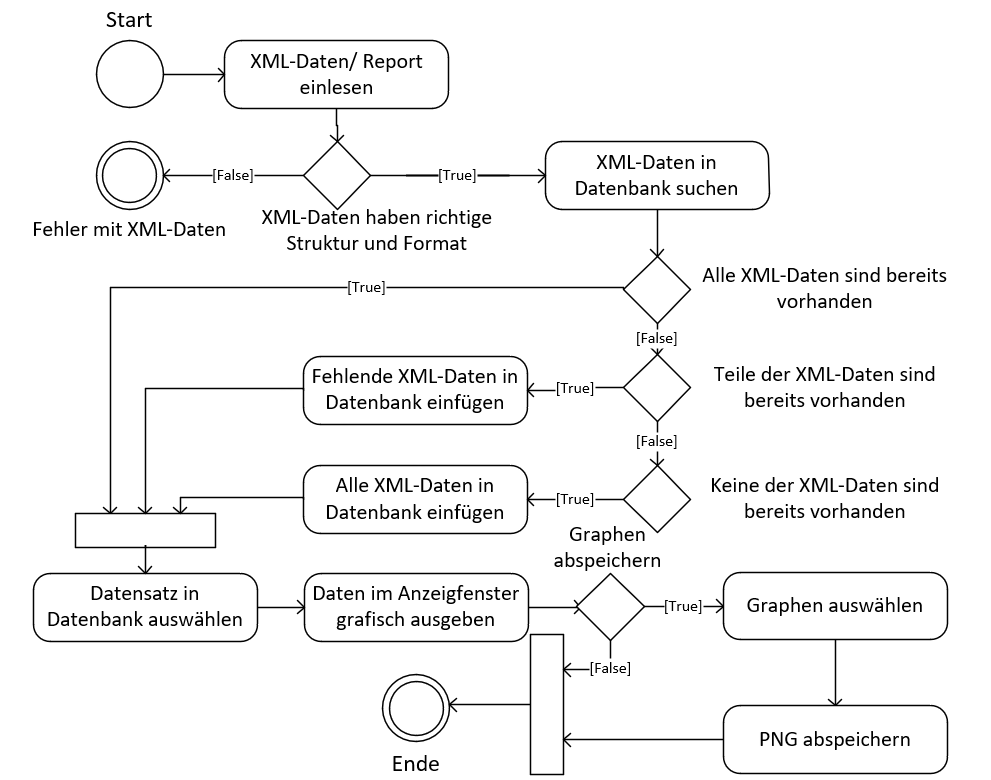
\includegraphics[width=0.95\textwidth]{Grafiken/Ablaufdiagramm}
    \caption{Grundlegedes Ablaufdiagramm der Nutzung der Web-Applikation}
    \label{fig: Grundlegedes Ablaufdiagramm der Nutzung der Web-Applikation}
    {Quelle: Eigene Darstellung mit Microsoft Visio}
\end{figure}
\subsection{Analyse der generierten XML-Berichte und bestehenden Strukturen}
\label{subsec:analyse-der-generierten-xml-berichte-und-bestehenden-strukturen}

In diesem Unterkapitel wird der Aufbau der automatisch
generierten Testberichte aus dem Teststand und der vorhandenen Ausgabe- und Speicherstruktur
erläutert. Dies ist relevant für die Erstellung der Datenbank und das
Verständnis der Ein- und Auslesefunktionen der Web-Applikation.

\subsubsection{XML-Berichtsstrukturschema}

Die vom Teststand automatisch generierten
Berichte folgen einem konstanten Strukturschema, welches sich bis zu einer
gewissen Ebene der XM-Struktur in jedem Bericht wiederholt. Wie im Kapitel „Grundlagen“
beschrieben, kann ein Element Attribute, andere Elemente und einen Inhaltswert beinhalten.

Das Stammelement heißt in allen automatisch
generierten Berichten „test“ und besitzt immer das Attribut „id“. Die Zahl in
diesem Attribut beschreibt den Typ des \ac{DUTs} die in diesem Test geprüft wurden.

Das Stammelement hat die Unter- bzw.
Kinderelemente „info“, „testbench“, „string“ und dreimal „testmodule“. Diese
Elemente haben wiederum alle weiter Unterelemente und Attribute.

Jedes der Elemente „testmodule“ hat ein Attribut
„name“, durch welches Sie unterschieden werden können. Das Element „string“ hat
ein Namensattribut mit der Bezeichnung „test sequence status“. Der Inhalt
dieses Elementes gibt an, ob der Test erfolgreich abgeschlossen wurde oder ob
es einen Fehler bzw. eine Grenzüberschreitung von Messwerten gab.
Die hier genannten eigenschaften sind in der Abbildung \ref{fig: Direkte Kinderelement unter Stammelement} zu erkennen.

\begin{figure}[H]
\centering
\begin{minipage}{0.95\textwidth}
\begin{lstlisting}[language=XML]
<?xml version="1.0" encoding="UTF-8"?>
    <test id="124">
    <info></info>
    <testbench></testbench>
    <testmodule name="DriverConsumptionTest"></testmodule>
    <testmodule name="PulseTest FSW L"></testmodule>
    <testmodule name="XPowerTest"></testmodule>
    <string name="test sequence status">
        Test sequence successfully finished.</string>
    </test>
\end{lstlisting}
\end{minipage}
\caption{Direkte Kinderelement unter Stammelement}
\label{fig: Direkte Kinderelement unter Stammelement}
    {Quelle: Eigene Darstellung}
\end{figure}


Das Element „info“ enthält in seinen Unterelementen die allgemeinen Testinformationen, wie die Startzeit des Tests,
die Typen-ID, die Konfigurationsbezeichnung des Teststandes, die Bezeichnung des angeschlossenen Carriers und die
Seriennummern des \ac{DUTs}. Diese Elemente haben keine Unterelemente und sind alle mit einem Namensattribut und einem Inhalt definiert.
Für die genauen Bezeichnungen und Struktur siehe Abbildung \ref{fig: XML-Strukturbeispiel Info-Element}

\begin{figure}[H]
\centering
\begin{minipage}{0.95\textwidth}
\begin{lstlisting}[language=XML]
<info>
	<string name="Time">2023-09-21_08:36:33</string>
	<string name="Material_number">124</string>
	<string name="Configuration">L_3DUT_3P1Q</string>
	<string name="ID_Carrier_left">Carrier 1</string>
	<string name="ID_DUT_R">10-29550</string>
	<string name="ID_DUT_S">10-29396</string>
    <string name="ID_DUT_T">10-29482</string>
</info>
\end{lstlisting}
\end{minipage}
\caption{XML-Strukturbeispiel Info-Element}
\label{fig: XML-Strukturbeispiel Info-Element}
    {Quelle: Eigene Darstellung}
\end{figure}

Die Teststandbezeichnung und die Versionen der Hard- und Software werden im Element „testbench“ gespeichert.
Diese Elemente enthalten auch keine weiteren Unterelemente und sind alle mit einem Namensattribut und einem Inhalt versehen.
Die genauen Bezeichnungen und die Struktur sind in Abbildung \ref{fig: XML-Strukturbeispiel Testbench-Element} zu sehen.

\begin{figure}[H]
\centering
\begin{minipage}{0.95\textwidth}
\begin{lstlisting}[language=XML]
<testbench>
	<string name="Testbench_name">USTB_DtWind</string>
	<string name="Testbench_HW_revision">V1.5</string>
	<string name="Version_GUI">V1.4.1</string>
    <string name="Version_controller">V1.3.2</string>
</testbench>
\end{lstlisting}
\end{minipage}
\caption{XML-Strukturbeispiel Testbench-Element}
\label{fig: XML-Strukturbeispiel Testbench-Element}
    {Quelle: Eigene Darstellung}
\end{figure}


Die Testmodule-Elemente sind alle nach dem gleichen Schema aufgebaut. Die ersten Unterelemente enthalten Grundinformationen
zu dem Status des Testmoduls, der Tages- und Uhrzeit des Tests und welche Versionen davon verwendet wurden.
Danach befinden sich noch drei weitere Elemente im Element „module“.
Diese Elemente heißen „Phase_U“, „Phase_V“ und „Phase_W“.
Sie besitzen kein Namensattribut.
Diese enthalten die Parameter und die Messdaten für die DUTs. Jede Phase enthält die Messwerte für ein DUT.
Somit besitzen alle Module unter dem Element „Phase_U“ die Messwerte und Parameter für den ersten DUT, dessen Seriennummer
unter dem Element mit dem Namensattribut „ID_DUT_R“ in Abbildung \ref{fig: XML-Strukturbeispiel Info-Element} zu finden ist.

In dem Element „parameters“, welches in jedem Phasenelement vorkommt, befinden sich die voreingestellten Rahmbedingungen
und Anforderungen für das Testmodul. Diese enthalten alle ein Namensattribut und einen Inhalt.

Die Elemente unter dem Eintrag „measurements“ enthalten die Messdaten der Testmodule. Sie haben oft noch extra Attribute
wie „min“ oder „max“, welche die Toleranzgrenzen beschreiben. Diese Toleranzgrenzen zeigen, in welchem Bereich der jeweilige
Elementinhalt angesiedelt sein muss, um kein positives bzw. fehlerfreies Ergebnis zu erzeugen.
Die meisten Attributswerte finden sich schon in den Parametern wieder und sind somit doppelt im Bericht zu finden.
Nur bei den Floatblock-Elementen, also Elementen mit der Bezeichnung Floatblock, sind besondere Attribute zu finden,
welche nicht gedoppelt vorkommen.
Diese Elemente umfassen zusätzlich die Attribute „size“ und „duration“, welche die Anzahl der in dem Inhalt enthaltenen
Floatwerte und die Dauer der Werteaufnahme angeben.
Diese sind für die grafische Darstellung besonders relevant.

Dies auf der Phasenebene: Treten keine Veränderungen in der XML-Struktur auf, variieren lediglich die Elemente unter den
Phasenelementen von Bericht zu Bericht etwas.
Die beträchtliche Ausnahme von dieser Regel bilden die Berichte, bei denen ein Fehler aufgetreten ist oder sogar der
Testvorgang abgebrochen wurde. Bei diesen Berichten hört die XML-Struktur bei den fehlgeschlagenen Testmodulen schon auf.
Der Testbericht ist aber in sich geschlossen. Das bedeutet, die XML-Struktur ist vollkommen und kann von einem XML-Parser eingelesen werden.
Es befinden sich nur weniger Testmodul-Elemente in dem Bericht und im Element für den Testsequenzstatus ist folgender Inhalt
enthalten: „Test sequence finished with errors.“ Zudem wird bei dem Testmodul, bei dem der Fehler aufgetreten ist, unter
dem Element mit dem Namen „Testresult“ ein Fehlercode und seine Bedeutung ausgegeben. In Abbildung \ref{} ist ein
Beispiel für einen Bericht, welcher beim ersten Testmodul einen Fehler ausgegeben hatte.
Bei einem Ausfall eines der zu testenden DUTs gibt es die Besonderheit, dass die anderen noch funktionsfähigen DUTs
keine weiteren Datenaufnahmen mehr machen können. Denn das System benötigt alle drei Phasen, um den Test durchzuführen.
Die XML-Struktur ist in sich geschlossen, aber es werden keine Daten von den anderen DUTs mehr aufgenommen.








\subsection{Datenbankdesign und Strukturkonzeption}
\label{subsec:datenbankdesign-und-strukturkonzeption}
\input{Kapitel/2. Hauptteil/3. Analyse und Konzeption/3.4 Grundkonzept des Benutzeroberflächen-Design}
\subsection{Entwurf der Applikationsarchitektur}
\label{subsec:entwurf-der-applikationsarchitektur}


Der Entwurf der Applikationsarchitektur bildet die konzeptionelle Grundlage für die technische Umsetzung der entwickelten Web-Applikation.
Das Ziel ist es, eine Struktur zu schaffen, die modular, wartbar und erweiterbar ist, und die gleichzeitig den funktionalen Anforderungen gerecht wird und sich in die bestehende Systemlandschaft integrieren lässt.
Die Architektur der Anwendung ist schichten- und komponentenorientiert aufgebaut und nutzt das Webframework Flask, welches eine klare Trennung zwischen der Präsentations-, Logik- und Datenhaltungsschicht ermöglicht.


\subsubsection{Architekturübersicht}

Die Applikation soll als serverbasierte Webanwendung im Client-Server-Modell funktionieren.
Das bedeutet: Während der Server die Datenverarbeitung, -speicherung und -bereitstellung übernimmt, ermöglicht der Client über den Webbrowser die Darstellung und Interaktion.
Die Anwendung ist in mehrere Schichten gegliedert, zu denen man die einzelnen Programmteile zuordnen kann.
Die Anwendung wird in folgende Schichten gegliedert:

\begin{itemize}
\item Präsentationsschicht (Frontend): Bereitstellung der Benutzeroberfläche über HTML-Templates, CSS und JavaScript.

\item
Applikationslogik (Backend): Implementierung der Geschäftslogik, Steuerung des Datenflusses und Verarbeitung der XML-Dateien.

\item
Datenhaltungsschicht: Persistente Speicherung der extrahierten Mess- und Gerätedaten in einer relationalen Datenbank mittels ORM.

\end{itemize}

Ein schematisches Architekturdiagramm dieser Struktur ist in Abbildung \ref{fig:arch_minimal} dargestellt.

\begin{figure}[H]
    \centering
    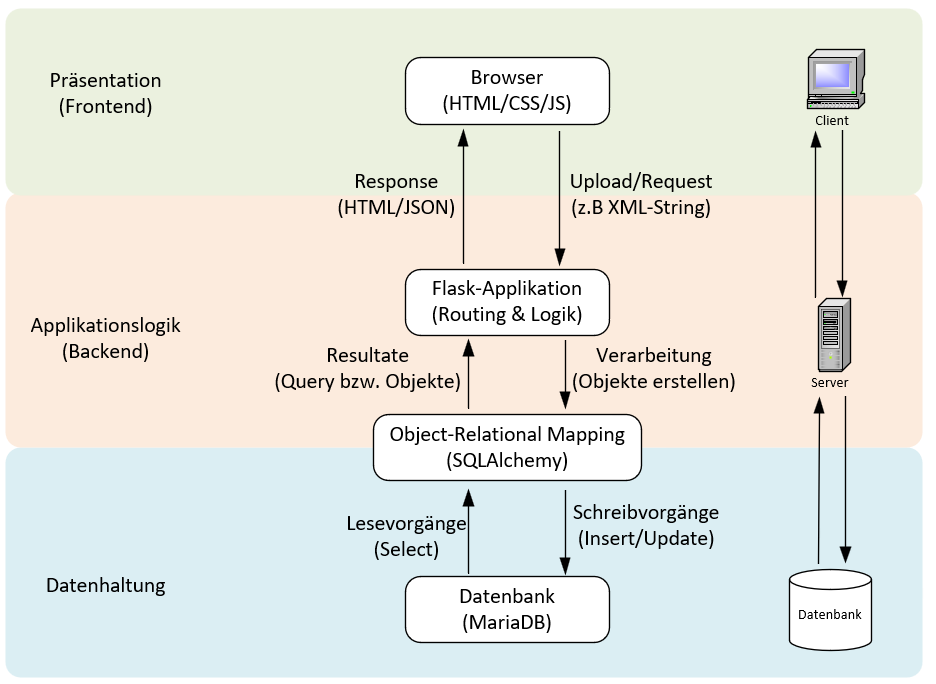
\includegraphics[width=0.95\textwidth]{Grafiken/Architekturdiagramm}
    \caption{schematisches Architekturdiagramm der Applikation}
    \label{fig:arch_minimal}
    {Quelle: Eigene Darstellung mit Microsoft Visio}
\end{figure}

\subsubsection*{Präsentationsschicht}

\begin{figure}[H]
  \centering
    \begin{minipage}{0.8\textwidth}
    \small
    Die Abbildung zeigt den Aufbau der Flask-Applikation.
    Im Verzeichnis \texttt{blueprints} befinden sich die einzelnen Routen-Module,
    während im Ordner \texttt{models} die Datenbankmodelle definiert sind.
  \end{minipage}
  \begin{minipage}{0.2\textwidth}
    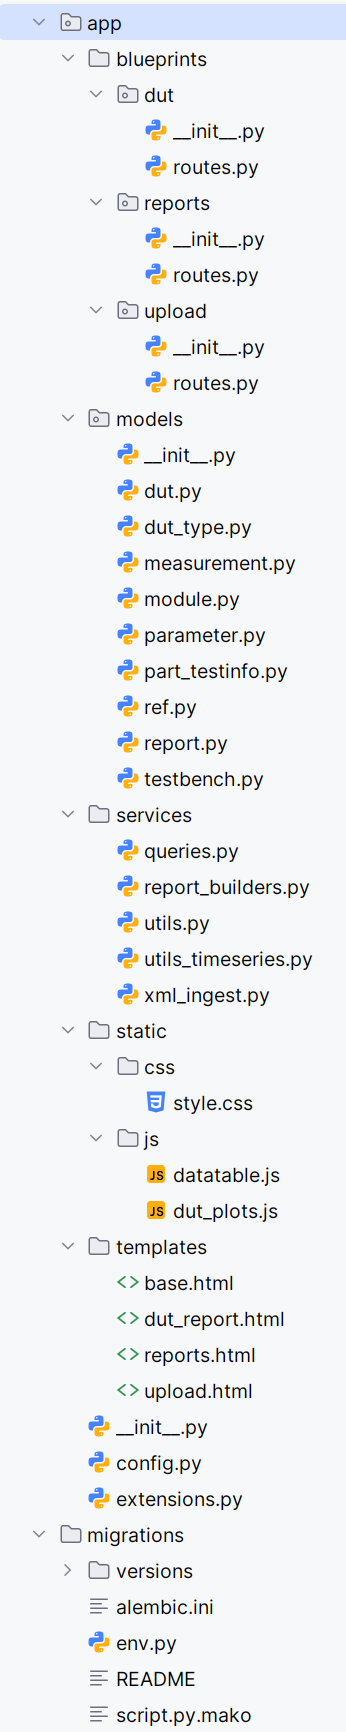
\includegraphics[width=0.9\textwidth, height=0.8\textheight, keepaspectratio]{Grafiken/App-Ordnerstruktur.png}
    \caption{Verzeichnisstruktur der Flask-Applikation}
    \label{fig:app-structure}
  \end{minipage}\hfill

\end{figure}

Die Präsentationsschicht besteht aus einer Kombination aus HTML-Templates und statischen Ressourcen (CSS, JavaScript), die im Verzeichnis templates/ bzw. static/ abgelegt sind.


\begin{itemize}

\item
Die Templates upload.html, reports.html und dut\_report.html bilden die Kernseiten der Weboberfläche.

\item
Statische Dateien wie style.css und dut\_plots.js dienen der Gestaltung und der interaktiven Darstellung von Messergebnissen.

Die Kommunikation mit der Logikschicht erfolgt über die definierten \textit{Flask Blueprints}, die als modulare Controller agieren.

\end{itemize}

\subsubsection*{Applikationslogik}

Die zentrale Geschäftslogik ist in modularen \textit{Blueprints} und \textit{Service-Komponenten} realisiert.

Die drei Blueprints upload, reports und dut kapseln die jeweiligen Funktionsbereiche:

\begin{itemize}

\item
upload: Einlesen und Validieren von XML-Dateien.

\item
dut: Verarbeitung und Anzeige der Daten eines „Device Under Test“.

\item
reports: Zusammenstellung und Ausgabe von Auswertungen.

\end{itemize}

Unterstützt werden diese durch das Modul services/, das die eigentliche Logik zur Datenverarbeitung bereitstellt:

\begin{itemize}

\item
xml\_ingest.py übernimmt das Parsen und Einlesen der XML-Daten.

\item
queries.py enthält vordefinierte Datenbankabfragen.

\item
utils.py und utils\_timeseries.py stellen Hilfsfunktionen zur Verfügung, z. B. zur Zeitreihenanalyse und Datenaufbereitung.

\item
report\_builders.py dient der Erstellung und Formatierung von Report-Daten für die grafische Darstellung.

\end{itemize}

Die Applikationslogik wird über die Datei run.py initialisiert, welche den Flask-Server startet und die Anwendungskonfiguration aus config.py einliest.


\subsubsection*{Datenhaltungsschicht}

Die Datenhaltung erfolgt über ein relationales Datenbanksystem, das über das Flask-eigene \textit{SQLAlchemy ORM} angebunden ist.

Die Datenmodelle sind im Verzeichnis models/ definiert und bilden die logischen Entitäten der Prüfanlage ab, darunter:

\begin{itemize}

\item
dut.py (Device Under Test)

\item
measurement.py (Messdaten)

\item
parameter.py (Prüfparameter)

\item
testbench.py, module.py und ref.py (Referenzdaten und Prüfaufbau)

\end{itemize}

Die Beziehungen zwischen den Modellen ermöglichen eine strukturierte und relationale Abbildung der Prüfdaten, wodurch eine effiziente Abfrage und Analyse möglich ist.

Migrationen werden mit \textit{Alembic} verwaltet, wie das Verzeichnis migrations/ zeigt.



\subsubsection{Kommunikation und Datenfluss}

Alles startet mit dem Hochladen einer XML-Datei über die Weboberfläche.
Der Blueprint upload übergibt die Datei an das Modul xml\_ingest, welches die XML-Struktur analysiert, relevante Informationen extrahiert und sie über die Datenmodelle in der Datenbank speichert.
 Die über den Blueprint reports oder dut gespeicherten Daten können anschließend abgerufen und visuell über die Templates dargestellt werden.
 Die Schichten kommunizieren ausschließlich über klar definierte Schnittstellen und ORM-Modelle, was eine lose Kopplung und eine hohe Wartbarkeit ermöglicht.











%! Author = jbf
%! Date = 31.07.25

\newpage
\section{Implementierung}
\label{Implementierung}

\subsection{Einlesen und Verarbeiten von XML-Daten}

\subsection{Implementierung der Datenbank}

\subsection{Entwicklung der Benutzeroberfläche}

\subsection{Technische Details zur Visualisierung}


%! Author = jbf
%! Date = 31.07.25

\newpage
\section{Integration und Test}
\label{Integration und Test}

\subsection{Einbindung in die bestehende Systemlandschaft}
\input{Kapitel/2. Hauptteil/5. Integration und Test/5.2 Testmethoden und Durchführung.tex}
\subsection{Ergebnisse der Testmethode}
\label{subsec:ergebnisse-der-testmethoden}

%------------------------------------------------------------------------------------------------------
%3. Schluss
%------------------------------------------------------------------------------------------------------
%! Author = jbf
%! Date = 31.07.25


\newpage
\section{Fazit und Ausblick}
\label{Fazit und Ausblick}

\subsection{Zusammenfassung der Ergebnisse}

\subsection{Kritische Bewertung}

\subsection{Möglichkeiten für zukünftige Erweiterungen}
\newpage
%------------------------------------------------------------------------------------------------------
%Einstellungsänderungen der Seitenzahlen zu kleine römisch Zahlen
%------------------------------------------------------------------------------------------------------
\renewcommand{\thesection}{\roman{section}}
\pagenumbering{roman}
\ohead[\pagemark]{}
\setcounter{section}{0}
%------------------------------------------------------------------------------------------------------
%Literaturverzeichnis
%------------------------------------------------------------------------------------------------------
\newpage
\addcontentsline{toc}{section}{Literaturverzeichnis}
\printbibliography
\newpage
%------------------------------------------------------------------------------------------------------
%Anhangsverzeichnis
%------------------------------------------------------------------------------------------------------
\section*{Anhangsverzeichnis}
\addcontentsline{toc}{section}{Anhangsverzeichnis}
\newpage
%------------------------------------------------------------------------------------------------------
%Erklärung
%------------------------------------------------------------------------------------------------------
\newpage
\section{Erklärung}
\label{sec:erklarung}
%\section*{Erklärung}
%\addcontentsline{toc}{section}{Erklärung}
\label{sec:erklärung}

Hiermit erkläre ich, dass ich die von mir eingereichte Bachelor- / Masterarbeit
„Datenverarbeitung und Visualisierung von Umrichter-Testbench-Daten“ selbständig und nur unter Verwendung der
angegebenen Quellen und Hilfsmittel angefertigt habe.
\\
\\
Ort und Datum: Drelsdorf, 27.10.2025
\\
\\
\\
\\
persönliche Unterschrift
\\
\\
\\
\\
Jon Feddersen


\medskip
\noindent\textbf{Zusatz zur Nutzung von KI-Assistenzsystemen}\\
Im Rahmen der Erstellung dieser Arbeit habe ich KI-gestützte Assistenzwerkzeuge
(\emph{QuillBot Grammar Checker} und \emph{ChatGPT})
\emph{ausschließlich} zu folgenden Zwecken eingesetzt:
(i) Rechtschreib- und Grammatikprüfung,
(ii) sprachliche Glättung und stilistische Hinweise zu von mir verfassten Textpassagen,
(iii) Recherchehilfe sowie Vorschläge zur Strukturierung/Gliederung.

Es wurden \emph{keine} inhaltlich tragenden Texte, Abbildungen oder Tabellen von KI-Systemen generiert und unverändert übernommen. Sämtliche inhaltlichen Aussagen, Formulierungen und Ergebnisse stammen von mir.
Alle verwendeten Quellen (einschließlich solcher, auf die KI-Werkzeuge ggf. hingewiesen haben) wurden von mir eigenständig geprüft, bewertet und ordnungsgemäß zitiert.

%------------------------------------------------------------------------------------------------------
%Dokument-End
%------------------------------------------------------------------------------------------------------
\end{document}
%------------------------------------------------------------------------------------------------------

